\documentclass[a4paper, 11pt]{article}
\usepackage[T1]{fontenc}
\usepackage[utf8]{inputenc}
\usepackage{natbib}
\usepackage{array}
\usepackage{anyfontsize}

\usepackage[margin=1.25in]{geometry}
\usepackage{hyperref} % links
\usepackage{parskip} % proper paragraphs, no indentation
\usepackage{pdfpages} % add non-plagiarism statement

% For showing the month + year only as the date:
\usepackage[en-GB]{datetime2}
\DTMlangsetup{showdayofmonth=false}

\usepackage{xcolor}

% This is used in the PDF meta data
\title{Moving beyond the Bechdel-Wallace test: using NLP to study gender representation in animated television shows}
\author{Alex Valisu}
\date{\today}
\setlength{\parindent}{1em}

\begin{document}
\newcolumntype{C}[1]{>{\centering\arraybackslash}m{#1}}
\newcommand\tablefont{\fontsize{7pt}{8pt}\selectfont}

% The actual title page of your thesis:
\begin{titlepage}
\begin{center}
\vspace*{.15\textheight}
{\Large Bachelor's Thesis}
\vspace{2em}

\vspace{0.6cm}
{\bfseries\huge
Moving beyond the Bechdel-Wallace test: using NLP to study gender representation in animated television shows
}\\[1cm] 
\vspace*{.05\textheight}
 
\begin{minipage}[t]{0.49\textwidth}
\begin{flushleft} 
{\large
\textit{Author}\\
Alex Valisu}\\
\href{mailto:alex.valisu@student.uni-tuebingen.de}{\textit{alex.valisu@student.uni-tuebingen.de}}\\
\end{flushleft}
\end{minipage}
\begin{minipage}[t]{0.49\textwidth}
\begin{flushright}
{\large
\textit{Supervisor}\\
Zarah Leonie Weiss}\\
\href{mailto:zweiss@sfs.uni-tuebingen.de}{\textit{zweiss@sfs.uni-tuebingen.de}}\\
\end{flushright}
\end{minipage}\\

\vfill

A thesis submitted in partial fulfilment\\
of the requirements for the degree of\\[2mm]
{\large Bachelor of Arts}\\
in\\[1mm]
{\large International Studies in Computational Linguistics}

\vspace*{.1\textheight}

{\large Seminar für Sprachwissenschaft\\
Eberhard Karls Universität Tübingen

\vspace{1em}
\today}
\end{center}
\end{titlepage}

% No page numbering for the abstract, the anti-plagiarism statement and the table of contents.
\pagenumbering{gobble}

\newpage

\includepdf[pages=-]{antiplagiat}

\newpage
\begin{center}
\section*{Abstract}
\end{center}
This thesis analyzes the transcribed dialogue of 16 different animated television shows in order to gauge the state of their gender representation on both a surface level and an in-depth level. A corpus of 1 803 individual speaker-annotated episode transcripts was collected and appropriately transformed for the purpose. The first part of the analysis uses statistical metrics to gauge the quantity of representation such as the proportional number of words spoken by each gender, the proportional number of speakers, an average number of words spoken by a speaker, and a variance of such statistics over the course of individual episodes. The second part focuses on natural language processing, namely co-reference analysis of the source material, in order to gauge the quality of representation. Additionally, as the majority of the analysis was performed using self-developed automatic tools, or is achievable through publically available tools such as the CoreNLP pipeline \citep{manning-EtAl:2014:P14-5}, this thesis forms the basis for further analyses of larger scope.

\newpage
\begin{center}
\section*{Acknowledgements}
\end{center}
First and foremost, I would like to thank my supervisor Zarah Weiss, not only for her great advice and guidance throughout writing this thesis and making me interested in the topic in the first place, but also for her understanding and for making me feel the safest I have ever felt during my university years.

I would also like to thank my partner and my friends for supporting me all the way through this process, being interested in my work, happily listening to my enthusiastic ramblings, and cheering me on when I needed it the most. Without you, I never would have had the strength to do this.

Finally, I would like to express my gratitude to my family, without which I never would have had an opportunity to study abroad and I never would have had the chance to write this thesis. Thank you for backing me up in my dreams.

\newpage
\tableofcontents
\listoftables
\listoffigures
\newpage

\pagenumbering{arabic}

\section{Introduction}
Art in its many shapes and forms is and always has been a core pillar of the world, serving as a form of expression, entertainment, respite and activism all at once. All art inherently reflects a set of cultural, moral and political values, either intentionally or not (as a lack of active statements in a work of art is a statement within itself), as art is a reflection of the artist, and no human being is apolitical or lacking any sort of values or convictions. It is therefore clear that works of art spread the values and ideals embedded in them onto its consumers, and at the very least give those values space in the public discussion, make them heard, and potentially even spread them and influence the world further. Such ideals are not necessarily overtly shown, and can manifest themselves in relatively minute or inconspicuous aspects of the work of art. With one of such values comes the idea of representation, the extent to which different groups of characters or different cultures appear, or are represented, in a work of art (such as gender, race, sexuality representation), and the way in which such characters or cultures are painted -- its quality (positive, neutral or negative representation of a group). It is important to note that lacking, insufficient or negative representation is not necessarily a product of malicious intent, and can simply be caused by misinformation or lack of education on the specific topic -- and in such cases, providing accurate statistical analyses on the subject can influence future representation in the matter, and is a form of education, not necessarily criticism. A representation of a group can influence the extent to which such a group is normalized over time by the majority population (its appearance being viewed as standard or normal, not a purposeful inclusion or a deviation from norm), and by extension helps members of such group feel included in the larger body of society. One can study many distinct representation groups, however, this thesis focuses on the idea of gender representation (the amount different genders make an appearance in a work of art, and the quality of such appearances).

First making its appearance in a 1985 comic strip "The Rule" in \textit{Dykes to Watch Out For} \citep{bechdel}, the Bechdel-Wallace test reads as follows: does a piece of media have at least two women in it who talk to each other about something other than a man? This question can be further separated into three sub-questions that have to be further analyzed separately: 1) does the work in question contain at least two women, 2) who talk to each other, 3) about something other than a man? The test aims to investigate a more complex issue with regards to gender representation than simple surface statistics, as a work of art can feature many non-male characters while failing to provide them with any depth, complexity, goals or stories of their own, which is a flaw a more superficial test might not be able to uncover. It is important to note that the Bechdel-Wallace test, while measuring the interactions of female characters more in-depth, is in no shape or form meant to be an end-all-be-all evaluation of a work of art \citep{zeisler}. Since it serves more of a first impression purpose, or a basis for further examination, this thesis aims to take over the concepts of the test and apply them to the work of art as a whole, or more specifically, to extend the simple yes/no result of the Bechdel-Wallace test into a more nuanced and detailed analysis across the whole work in question and to extract statistics more relevant to a proper evaluation of gender representation.

In addition to providing statistics about gender representation, this thesis also helps expand the field of computational linguistics in this specific area. A speaker-annotated corpus was composed for the purposes of this thesis, and different statistical methods were explored with regards to gender analysis. Natural language processing tools were used in order to analyze the co-reference of the corpus -- which additionally included an evaluation of several types of models with regards to the highly specific format of the source data. Such gained knowledge has the potential to be used in further projects, especially in those closely related in topic.

With countless works of art created every single day, this thesis settles on a narrow selection of works to focus on: animated television shows (further referred to simply as television shows, shows, or cartoons). Given the origins of the Bechdel-Wallace test, which spoke of movies, animated television shows align in spirit with the test and its original intent. In addition, while gender representation is without a doubt an important topic in any medium, it is arguably the most essential with art primarily aimed at, or consumed by, children who are easily impressionable. While this thesis cannot accurately represent and evaluate data from a massive sample of shows to capture a highly accurate trend across the entire spectrum (as the needed source data is largely not publically available for a critical mass of cartoons, and is time-consuming to collect from the raw footage), it aims to create an in-depth analysis of a diverse sa	mple, and to provide automated tools able to largely handle further analyses on their own given the appropriate data.

This thesis aims to answer the first two sub-questions of the Bechdel-Wallace test for several animated television shows, and dives deeper into the complex aspects of gender representation in the medium. The television shows in question were hand-picked with a focus on diversity in airing times, creators and age ratings, aiming to cover a spectrum as wide as possible within the scope of the thesis. It is structured as follows: section 1 mentions related work with regards to both the Bechdel-Wallace test, and the natural language processing methods used in later sections. Section 2 explains the data selection, gathering and wrangling process, and shows an overview of the data and its metadata used in the analysis process. Methods as well as automated tools used to gather important statistics about the data are subsequently reported in section 3, and its results and analyses are shown in section 4. Finally, section 5 concludes the thesis.

\section{Related Work}

\subsection{Bechdel-Wallace Test}
What has later become known as the Bechdel-Wallace test, an idea put into paper by Alison Bechdel thanks to the inspiration from Liz Wallace, almost certainly has its origins in a quote from Virginia Woolf \citep{testy}:

\begin{center}
\textit{"All these relationships between women, I thought, rapidly recalling the splendid gallery of fictitious women, are too simple. ... And I tried to remember any case in the course of my reading where two women are represented as friends. ... They are now and then mothers and daughters. But almost without exception they are shown in their relation to men. It was strange to think that all the great women of fiction were, until Jane Austen's day, not only seen by the other sex, but seen only in relation to the other sex. And how small a part of a woman's life is that ..."} \citep{woolf}
\end{center}

The comic strip (as displayed in Figure \ref{fig:bechdel}), has since its first publishing grown into a large phenomenon that has not only attracted praise and criticism, but also further derivations. A complete dive into the consequences of the comic strip would require a thesis on its own, and thus only a short summary is provided in this subsection.

\begin{figure}[h!]
  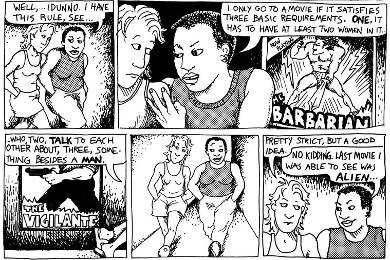
\includegraphics[width=\linewidth]{figures/bechdel.jpg}
  \caption{The first appearance of what was later dubbed the Bechdel-Wallace test. \citep{bechdel}}
  \label{fig:bechdel}
\end{figure}

The Bechdel-Wallace test has made a large cultural impact, with media outlets making a notice of it and frequently using or mentioning the test in their publications. However, mainstream usage was not the only area the test was used in, as seen by the Swedish Film Institute incorporating the test into some of their ratings \citep{swedes}. Work has also been made in the field of automating the application of the Bechdel-Wallace test, as is shown in \citet{otherbechdelresearch}.

However, the Bechdel-Wallace test has never meant to be an all-encompassing test of the inclusivity of a piece of media, and as stated in \citet{zeisler}, the test's utility has been elevated beyond its original intention. While it is possible to apply the rules as a type of litmus test to pieces of media to gauge the surface level of inclusivity, it is important to note that passing the Bechdel-Wallace test does not equate with being inclusive and feminist. It is reasonable to object to the attention the test is given and the status of end-all-be-all test that may be attributed to it, but it would be unjust to judge the test itself for it, as it was never designed to be so.

\subsection{Co-reference Analysis}
In the instance where two different words or expressions in a text refer to the same object -- referent (e. g. in the sentence "\textit{Jane} said \textit{she} is ill," the words Jane and she refer to the same object, Jane), we are speaking about co-reference \citep{dictionary}. As such a relationship between expressions can be complicated and not always clear (and not even always unambiguous), co-reference resolution attempts to find such bound expressions, either for the purpose of further analysis, or for the purpose of annotation. Its uses are wide, as many linguistic tasks depend on it, ranging from the basic such as correctly understanding the source text in the first place, to more complex analyses and statistics, some of which will be explored later in this thesis. It is important to note that automatic co-reference analysis relies on other annotations in order to function. While this varies between models, in general co-reference analysis requires a type of parses, be it dependency or constituency parses.

As with many corpus analysis tasks, while it is possible to annotate co-reference resolution manually, many automated tools were developed for the purpose. There are three main branches of different models, namely deterministic, statistical and neural, and each have gone through their evolutions and inspirations. Since a full recount of the history of analyzing co-reference resolution could easily result in a full-length thesis on its own, this section aims to cover the topic briefly with outside sources for providing more in-depth information. Additionally, this section focuses on models trained for English, as that is the language the research of this thesis focuses on.

Described in detail in \citet{jurafsky}, co-reference pairs can be filtered out on the basis of several constraints, among which belong number agreement, where the two expressions should align in number (singular or plural), person and case agreement, gender agreement, syntactic rules, and others. This is only a first step, however, as while these methods can rule out possible expressions that do not align, a pair that passes through every filter is still not guaranteed to be co-referent. This issue is present with rule-based approaches in general, as the English language contains many ambiguities even for a human eye, and absolute precision is thus not always achievable.

Rule-based approaches have gone through meaningful development over the course of its existence. At first, the systems did not achieve good performance due to factors such as hand-tuning the weights of the models (one such early model can be seen in \citet{lappin}). Further information about early model propositions can also be found in \citet{baldwin}. At first, the realizations of such propositions involved single-pass models, which were later replaced by the use of multi-pass models \citep{raghunathan2010}. Such models consist of several different rule-based sieves which attempt to find a co-reference pair, and unresolved expressions trickle down into the subsequent sieves. Usually, sieves are sorted in order of coarseness, such that an exact-match sieve (which looks for strings that match each other) is applied first, with more specialized sieves being applied next. Further extensions of the model have been seen in \citet{lee11conllst}, such as the addition of multiple sieves and a post-processing step. In addition, multiple researches and improvements such as identifying singleton mentions \citep{recasens_demarneffe_potts2013} have been published since then.

As described in \citet{clark2015entity}, a development has been made to the co-reference resolution methods by working with clusters of mentions instead of simple pairs. With such approach, it was possible for earlier co-reference decisions to inform later ones (such as the aforementioned gender agreement, where a co-reference link between a name and a pronoun could establish the gender, and such decision could inform further co-reference links further in the text). Additionally, the model reduces the search space for possible links, and introduces several features which inform the decision to create a link, such as distance, string matching (borrowing from rule-based methods) and lexical, semantic and syntactic features.

With the rise of neural networks, such systems have penetrated even the subject of co-reference resolution. One such model is described in \citet{clark2016deep}, using mention-ranking at its core (scoring pairs of mentions on their likelihood of co-reference). Such a model can yet again be extended by working with clusters, and this including an entity-ranking model in addition to the mention-ranking one \citep{clark2016impr}. Overall, the field of co-reference resolution is a blooming one, and new methods, findings and improvements are frequent.

\section{Data}

\subsection{Corpus Profile}
The corpus composed for the purpose of this thesis, the detailed creation process of which is described later in this section, contains episode transcripts (speaker-annotated lines of dialogue complimented by out-of-character descriptions) of 16 animated television shows. In total, 1 803 individual episode transcripts are present, with a total number of 5 309 981 tokens collected, an average episode length of 2 945 tokens, and a standard deviation of 1 930. A detailed breakdown of the total number of tokens, the average number of tokens per episode transcript, and the standard deviation of each individual television show is available in Table \ref{tab:corpus}. A more detailed metadata table of the analyzed television shows is available in subsection \ref{dat:col} in Table \ref{tab:shows}.

\begin{table}[h!]
\centering
  \begin{small}
  \begin{tabular}{|| c | c | c | c ||}
  \hline
  Code & Total Token Number & Average Tokens/Episode & Standard Deviation \\
  \hline\hline
  ADV & 490 826 & 2 080 & 776 \\
  \hline
  ATL & 330 422 & 5 329 & 1 460 \\
  \hline
  CLW & 36 308 & 2 421 & 353 \\
  \hline
  DUC & 190 991 & 3 351 & 1 333 \\
  \hline
  FUT & 531 152 & 5 107 & 2 501 \\
  \hline
  GRA & 187 396 & 4 685 & 762 \\
  \hline
  GUM & 620 409 & 2 607 & 448 \\
  \hline
  KOR & 263 496 & 4 972 & 1 602 \\
  \hline
  MLP & 632 587 & 2 787 & 281 \\
  \hline
  OWL & 93 512 & 3 896 & 1 928 \\
  \hline
  PPG & 444 325 & 3 220 & 882 \\
  \hline
  RAM & 122 362 & 4 894 & 1 392 \\
  \hline
  SHE & 195 008 & 3 824 & 1 106 \\
  \hline
  SPO & 677 610 & 2 104 & 1 066 \\
  \hline
  STU & 411 959 & 2 203 & 839 \\
  \hline
  VOL & 81 618 & 3 401 & 1 930 \\
  \hline
  \end{tabular}
  \end{small}
  \caption{A breakdown of the total token number, average token number per episode, and standard deviation of each television show in the corpus.}
  \label{tab:corpus}
\end{table}

\subsection{Collection and Types} \label{dat:col}
In order to gather a sufficiently sized sample of data from a wide variety of television shows, it was deemed impossible to manually transcribe a statistically significant number of episodes and provide additional required metadata, such as speaker annotation. Additionally, official transcript data (a transcript being a rewriting of an episode's dialogue with speakers assigned to their respective lines, often with out-of-character descriptions included) is rarely available and in the case of select streaming platforms which offer their own subtitles, an export of such files is not possible. To solve this problem, data had to be gathered from fan-made wikis (a wiki being a topic-specific encyclopedia website). Due to not having access to official or self-produced data, special attention had to be put into assessing the reliability and accuracy of the given information provided by a non-official source.

Accounting for such time-intensive process of collecting data, and with the number of animated television shows existing in the world greatly exceeding the scope of any one singular paper, it was necessary to focus on a limited number of cartoons, and thus for as broad of a scope as possible within the limited data availability, metrics for selection had to be created to cover as many different types of television shows as possible. Surprisingly, a crucial metric such as popularity was hard to access, as the process was hindered both by the age of the cartoon -- and thus incomplete or missing viewer data, or data which fails to capture the general viewership trends across the years -- and also by the recent shift in television as a whole -- with many cartoons running in parallel or exclusively on streaming services instead of traditional television. With this in mind, while it was possible to use viewership and popularity to some extent to determine the shows for analysis, it was necessary to supplement those with other metrics. Determining it was important to focus on diversity (as a large number of television shows exploring similar space would provide skewed information about the cartoon scene as a whole), the metrics devised to capture a wide range of shows were as follows: 1) the main author, 2) the original network, 3) the original airing time, 4) the genre(s), and 5) the age rating.

\begin{table}[p!]
\centering
  \begin{tablefont}
  \begin{tabular}{|| >{\centering\arraybackslash}m{0.5cm}
        | >{\centering\arraybackslash}m{1.5cm}
        | >{\centering\arraybackslash}m{4cm}
        | >{\centering\arraybackslash}m{3cm}
        | >{\centering\arraybackslash}m{2cm} ||} 
  \hline
  ID\rule[-2ex]{0pt}{6ex} & Code\rule[-2ex]{0pt}{6ex} & Full Name\rule[-2ex]{0pt}{6ex} & Genre(s)\rule[-2ex]{0pt}{6ex} & Airing Time\rule[-2ex]{0pt}{6ex} \\
  \hline\hline
  1 & ADV & Adventure Time & \shortstack{ \\ Adventure, Comedy \\ Science Fantasy} & 2010 - 2018 \\
  \hline
  2 & ATL & Avatar: The Last Airbender & \shortstack{ \\ Action, Adventure \\ Fantasy} & 2005 - 2008 \\
  \hline
  3 & CLW & Star Wars: The Clone Wars & \shortstack{ \\ Action, Adventure \\ Science Fiction} & 2008 - 2020 \\
  \hline
  4 & DUC & DuckTales & \shortstack{ \\ Action, Adventure \\ Comedy} & 1987 - 1990 \\
  \hline
  5 & FUT & Futurama & \shortstack{ \\ Comedy, Sitcom \\ Science Fiction} & 1999 - 2013 \\
  \hline
  6 & GRA & Gravity Falls & \shortstack{ \\ Adventure, Comedy \\ Mystery} & 2012 - 2016 \\
  \hline
  7 & GUM & The Amazing World of Gumball & \shortstack{ \\ Comedy, Fantasy \\ Sitcom} & 2011 - 2019 \\
  \hline
  8 & KOR & Avatar: The Legend of Korra & \shortstack{ \\ Action, Adventure \\ Steampunk} & 2012 - 2014 \\
  \hline
  9 & MLP & \shortstack{ \\ My Little Pony: \\ Friendship is Magic} & Fantasy & 2010 - 2019 \\
  \hline
  10 & OWL & The Owl House & \shortstack{ \\ Fantasy \\ Horror Comedy} & 2020 - present \\
  \hline
  11 & PPG & The Powerpuff Girls & \shortstack{ \\ Action, Adventure \\ Superhero} & 1998 - 2005 \\
  \hline
  12 & RAM & Rick and Morty & \shortstack{ \\ Adventure, Comedy \\ Science Fiction} & 2013 - present \\
  \hline
  13 & SHE & \shortstack{ \\ She-Ra and the \\ Princesses of Power} & Action, Adventure & 2018 - 2020 \\
  \hline
  14\rule[-2ex]{0pt}{6ex} & SPO\rule[-2ex]{0pt}{6ex} & SpongeBob SquarePants\rule[-2ex]{0pt}{6ex} & Comedy\rule[-2ex]{0pt}{6ex} & 1999 - present\rule[-2ex]{0pt}{6ex} \\
  \hline
  15 & STU & Steven Universe & \shortstack{ \\ Action \\ Science Fantasy} & 2013 - 2019 \\
  \hline
  16 & VOL & Voltron: Legendary Defender & \shortstack{ \\ Action, Adventure \\ Science Fantasy} & 2016 - 2018 \\
  \hline
  \hline
  ID\rule[-2ex]{0pt}{6ex} & Age Rating\rule[-2ex]{0pt}{6ex} & Creator(s)\rule[-2ex]{0pt}{6ex} & Network(s)\rule[-2ex]{0pt}{6ex} & Episodes\rule[-2ex]{0pt}{6ex} \\
  \hline\hline
  1\rule[-2ex]{0pt}{6ex} & PG\rule[-2ex]{0pt}{6ex} & Pendleton Ward\rule[-2ex]{0pt}{6ex} & Cartoon Network\rule[-2ex]{0pt}{6ex} & 236\rule[-2ex]{0pt}{6ex} \\
  \hline
  2 & Y7 & \shortstack{ \\ Michael Dante DiMartino \\ Bryan Konietzko} & Nickelodeon & 62 \\
  \hline
  3 & PG & George Lucas & \shortstack{ \\ Cartoon Network \\ Disney} & 15 \\
  \hline
  4 & Y7 & \shortstack{ \\ Jymn Magon \\ Brad Landreth} & Syndication & 57 \\
  \hline
  5\rule[-2ex]{0pt}{6ex} & 14\rule[-2ex]{0pt}{6ex} & Matt Groening\rule[-2ex]{0pt}{6ex} & Fox, Comedy Central\rule[-2ex]{0pt}{6ex} & 104\rule[-2ex]{0pt}{6ex} \\
  \hline
  6\rule[-2ex]{0pt}{6ex} & Y7\rule[-2ex]{0pt}{6ex} & Alex Hirsch\rule[-2ex]{0pt}{6ex} & Disney\rule[-2ex]{0pt}{6ex} & 40\rule[-2ex]{0pt}{6ex} \\
  \hline
  7\rule[-2ex]{0pt}{6ex} & Y7\rule[-2ex]{0pt}{6ex} & Ben Bocquelet\rule[-2ex]{0pt}{6ex} & Cartoon Network\rule[-2ex]{0pt}{6ex} & 238\rule[-2ex]{0pt}{6ex} \\
  \hline
  8 & PG & \shortstack{ \\ Michael Dante DiMartino \\ Bryan Konietzko} & Nickelodeon & 53 \\
  \hline
  9\rule[-2ex]{0pt}{6ex} & Y\rule[-2ex]{0pt}{6ex} & Lauren Faust\rule[-2ex]{0pt}{6ex} & Discovery Family\rule[-2ex]{0pt}{6ex} & 227\rule[-2ex]{0pt}{6ex} \\
  \hline
  10\rule[-2ex]{0pt}{6ex} & Y7\rule[-2ex]{0pt}{6ex} & Dana Terrace\rule[-2ex]{0pt}{6ex} & Disney\rule[-2ex]{0pt}{6ex} & 24\rule[-2ex]{0pt}{6ex} \\
  \hline
  11\rule[-2ex]{0pt}{6ex} & Y7\rule[-2ex]{0pt}{6ex} & Craig McCracken\rule[-2ex]{0pt}{6ex} & Cartoon Network\rule[-2ex]{0pt}{6ex} & 138\rule[-2ex]{0pt}{6ex} \\
  \hline
  12 & 14 & \shortstack{ \\ Justing Roiland \\ Dan Harmon} & Adult Swim & 25 \\
  \hline
  13\rule[-2ex]{0pt}{6ex} & Y7\rule[-2ex]{0pt}{6ex} & Noelle Stevenson\rule[-2ex]{0pt}{6ex} & Netflix\rule[-2ex]{0pt}{6ex} & 51\rule[-2ex]{0pt}{6ex} \\
  \hline
  14\rule[-2ex]{0pt}{6ex} & Y7\rule[-2ex]{0pt}{6ex} & Stephen Hillenburg\rule[-2ex]{0pt}{6ex} & Nickelodeon\rule[-2ex]{0pt}{6ex} & 322\rule[-2ex]{0pt}{6ex} \\
  \hline
  15\rule[-2ex]{0pt}{6ex} & PG\rule[-2ex]{0pt}{6ex} & Rebecca Sugar\rule[-2ex]{0pt}{6ex} & Cartoon Network\rule[-2ex]{0pt}{6ex} & 187\rule[-2ex]{0pt}{6ex} \\
  \hline
  16 & Y7 & \shortstack{ \\ Lauren Montgomery \\ Joaquim Dos Santos} & Netflix & 24 \\
  \hline
  \end{tabular}
  \end{tablefont}
  \caption{A metadata table of the analyzed television shows.}
  \label{tab:shows}
\end{table}

The unavailability of official data and the need to rely on fan-made content has noticeably reduced the possible range of television shows, however, the selection still offered a large amount of variety. All 16 television shows used for the analysis along with their details can be found in Table \ref{tab:shows} under their specific three-letter codes, which are further used to uniquely identify them instead of their names. While the number of analyzed episodes per television show varies greatly, it was considered more beneficial to work with proportional analysis rather than gather a substantially smaller equally sized sample of each television show. Overall, a total of 1 803 episode transcripts were collected, with each individual transcript representing 10-25 minutes of raw episode footage. Individual episode transcripts were manually checked and deemed acceptable for use in the analysis depending on their completeness, accuracy and consistency. Unfinished transcripts or transcripts with partially or fully missing speaker labels were not considered for the analysis, but transcripts with missing out-of-character descriptions were deemed acceptable, as lack thereof only resulted in a larger amount of further manual work (specifically automatic gender determination, described further in subsection \ref{met:genan}), not a decrease in accuracy.

All source data in the form of individual transcript websites was manually gathered in the HTML format, as such collection followed by automatic text conversion and transcript extraction proved to be more efficient than manually locating transcript data within a webpage and exporting it into a TXT format. During the process, several different types of transcripts were also identified that had to be handled differently in the upcoming data wrangling process (described in subsection \ref{dat:datwran}). Including only the data deemed fit to be analyzed, meaning complete transcripts with fully annotated speaker information, the types appearing were as follows: 1) an in-line speaker annotation separated by a colon from their respective lines, with out-of-character descriptions sitting on a separate line in either round or square brackets (displayed in Figure \ref{fig:format1}), and 2) a table format, with the first column listing the speaker (or being empty in case of an out-of-character description), and the second column listing the respective lines (displayed in Figure \ref{fig:format2}).

\begin{figure}[h!]
  \centering
  \begin{small}
  \begin{tabular}{l}
  Speaker 1: "A sentence spoken by speaker 1. A second sentence spoken by speaker 1." \\
  An out-of-character description. A second line of the description. \\
  Speaker 2: "A sentence spoken by speaker 2. A second sentence spoken by speaker 2." \\
  \end{tabular}
  \end{small}
  \caption{An in-line formatting of the source data.}
  \label{fig:format1}
\end{figure}

\begin{figure}[h!]
  \centering
  \begin{small}
  \begin{tabular}{c | l}
  Speaker 1 & A sentence spoken by speaker 1. A second sentence spoken by speaker 1. \\
  \hline
   & An out-of-character description. A second line of the description. \\
   \hline
  Speaker 2 & A sentence spoken by speaker 2. A second sentence spoken by speaker 2. \\
  \end{tabular}
  \end{small}
  \caption{A table formatting of the source data.}
  \label{fig:format2}
\end{figure}

\subsection{Data Wrangling} \label{dat:datwran}
Data wrangling describes a process of transforming and filtering the collected raw data into data ready to be used for further tasks. It is crucial to determine the desired end-point and format of the data before beginning the wrangling process itself. For the purposes of this thesis, two different data wrangling processes were applied to the source data, with the latter process using the data from the former as its source. This was necessary, as the different analyses implemented further down the line required a separate format in order to function properly. However, even before such split could be made, the first step to be taken was a transformation of the source data to a unified format. With the high number of the source files, it was determined the best approach was transforming the data automatically using a self-developed script tailored for the purpose.

As the desired output format was a TXT file, it was determined the unified format should follow the one shown in Figure \ref{fig:format1}. Other available options for a TXT file (since a table format is not supported) was a comma-separated file (which would have the potential for a high level of disruptions, since the source data features a large number of commas), and a tab-separated file (which features the least amount of potential faultiness). It should be acknowledged that the chosen format has a slim potential for faultiness since colons do appear in the source format even in other contexts, however, due to the further handling of the data, it posed no risk of affecting the outcome of the analysis. A tab-separated format would be a better formatting choice from the point of additional workload in a vacuum, however, as the majority of the source data already corresponded to the colon-separated format, the minor faultiness would have already applied were the data transformed to a tab-separated format beforehand, and it was thus chosen to stay with the colon-separated format.

In order to change the formatting of the transcript, it was first required to isolate it from the rest of the webpage, as it featured additional information pertaining to the transcript but not being a direct part of it. As the individual wikis shared little consistency between each other, it was necessary to manually identify the markings used to differentiate transcripts from additional information for each television show separately, and to then subsequently divide the shows to smaller groups to be handled separately. In total, three such groups were devised, and each individual show was additionally checked to be converted into the proper format if necessary. Since a table format converted into plain text was represented as separate lines, special care had to be put into assigning each line to its rightful speaker, and to not mix those with out-of-character descriptions, other speakers' names, or other speakers' lines.

With all the individual episode transcripts following the format shown in Figure \ref{fig:format1}, the data was thus ready for gender analysis described in subsection \ref{met:genan} -- the reason for why this format was chosen for this particular analysis will also be described in this subsection, as well as the specific benefits to each individual method. However, co-reference resolution, described in subsection \ref{met:coref}, has a need for a more specific format of data, as the implemented automatic tools required a specific formatting in order to acknowledge for the present metadata, such as the annotated speakers. The reasoning for the used format (displayed in Figure \ref{fig:formatcoref}), as well as the process that led to devising such a format, will be described in the appropriate section, as it is necessary to first explore how automatic co-reference analysis and the specific tool used in this project work.

\begin{figure}[h!]
  \centering
  \begin{small}
  \begin{tabular}{l}
  Speaker 1 says: "A sentence spoken by speaker 1." \\
  Speaker 1 says: "A second sentence spoken by speaker 1." \\
  An out-of-character description. A second line of the description. \\
  Speaker 2 says: "A sentence spoken by speaker 2." \\
  Speaker 2 says: "A second sentence spoken by speaker 2." \\
  \end{tabular}
  \end{small}
  \caption{The formatting used for coreference resolution.}
  \label{fig:formatcoref}
\end{figure}

\section{Methods}

\subsection{Gender Analysis} \label{met:genan}

\paragraph{Gender Definition and Data Collection:}
In order to perform gender analysis, it was integral to at first establish the definition of gender used in this project, and to subsequently assign a gender group to each speaker. There are three groups of genders classified for the purpose of the following analysis: male, female, and non-binary (encompassing all genders falling outside of the gender binary, as well as genderless characters). It should be noted that sexless characters are not necessarily genderless and vice versa -- while gender and sex overlap for the majority of characters in the selected television shows, the analysis focuses on gender and ignores sex in case those two characteristics do not align with each other. As there rarely exists definitive data for each character, this thesis follows these guidelines in order of importance: 1) canonical gender provided either out-of-universe by the television show's creators, or in-universe inside of the show itself, and 2) if no such canonical information is provided, it is assumed pronouns he/him/his refer to male characters, she/her/hers refer to female characters, and singular they/them/their/theirs refer to non-binary or genderless characters. The names of all speakers were automatically gathered from all episode transcripts along with the total number of words spoken by that speaker, and subsequently exported into a separate file for further use.

To analyze any meaningful statistics about gender, the necessary first step was to devise a method to either manually or automatically assign a gender group to each individual speaker. Initially, it was planned to gather gender information by automatically searching the associated webpages of each individual character on their respective fan wikis. However, this process was hindered by several complications and eventually was deemed too faulty to use reliably. The largest flaw was the frequent mismatch of website names and character names used in the source transcript. In many cases, a character was referred to only by a part of their name, e.g. "Anakin" in place of "Anakin Skywalker". Additionally, many significant characters appeared in the transcript who either did not have an associated webpage (due to the incompleteness of the wiki itself, the character page policy of the given wiki, or simply due to several different mutually related characters sharing a single webpage), their gender was not listed on their website, or their name was in other ways different from the name of the webpage their character profile was located at. It was decided that while this method would be capable of producing sufficient results, it would also require heavy manual correction following the automatic search part (and the whole process would possibly become even more time-intensive than a fully manual approach), and thus a different approach was more likely to be suitable.

The method used in the final version of the project was an automated gender guesser accompanied by manual checking and filling in of missing information. Since a large portion of the source data contained out-of-character descriptions, it was possible to automatically extract an exact number of gender or pronoun mentions occurring in all instances of descriptions accompanying a specific character's lines using a self-developed script. With the guidelines established above, a statistic was established for every character and their gender was established based on the prevalent gender or pronoun usage. However, it is important to note this process is not definite, and requires subsequent manual check-up, as descriptions occasionally include mentions of genders or pronouns belonging to characters other than the speaker. While the guesser was mostly accurate (as mentions of the speaker occurred in larger numbers than mentions of other characters), several errors had to be manually corrected. In addition, the guesser was implemented solely for male and female genders, as the combination of non-binary genders being too infrequent in the source material and the large amount of noise generated by mistaking the plural "they" for the singular "they" has proven to decrease the accuracy of the guesser. A manual check-up was performed on the output data, correcting the gender of non-binary characters and inserting gender information for television shows whose transcripts lacked out-of-character descriptions. Additionally, it was chosen to only include named characters with more than 100 words (words being all alphanumeric sequences of characters separated by a whitespace) spoken across the entire television show, as characters below this threshold form a large percentage of speakers and a minuscule percentage of on-screen appearance, and have thus a high potential to bloat the amount of data needed to be manually inspected, and to skew the following statistics. The exclusion of non-named characters was made on the basis of both the high chance of smaller importance, as well as the possibility of one label belonging to more than one character, possibly to characters of differing genders. For example, a speaker referred to as "Guard" can possibly refer to several different guards even in the span of a single television show or a single episode, and it is possible those characters do not share a gender. Additionally, even if such a label only referred to a singular character, it would require a large amount of manual work examining the video footage of the given episode to determine the speaker gender (as non-named characters do not possess a webpage of their own on their respective wikis) for comparably minuscule gain (non-named characters tend to have a significantly smaller number of words spoken than named characters, as characters with a significant presence in the source material have most often been given names).

While non-binary representation is an aspect of gender representation worth investigating, the resulting data have shown very few results on the matter. No individual television show has contained more than a handful of non-binary or genderless characters according to the previously established criteria, and the majority of television shows contained none. With the acknowledgement non-binary representation is an important subject to study, and with the admittance the source material has proven to not contain enough data to include such a study in the following analysis, this thesis decides to only focus on the representation and relation of male and female genders from this point onward, and excludes all non-binary or genderless characters from its statistics.

\paragraph{Metrics and Statistics:}
Gender analysis can be performed in several ways, each one yielding a different type of information about the source material. This thesis aims to analyze the data from multiple different angles to form a larger picture about the state of gender representation and to answer several questions that can help shed more light into the exact specifics of the issue. It is important to note that because this subsection deals with no natural language processing tools and only works with raw numbers, the data gathered in this part of the analysis largely focuses on quantity over quality (the latter of which will be explored more thoroughly in subsection \ref{met:coref}). The first and most basic statistic that is possible to extract from the source data is comparing the total number of words spoken by all speakers of a given gender in one specific television show to the same statistic of a different gender, and providing the results for every cartoon separately (further referred to as \textit{words per gender}). With access to transcript data and without using actual episode video footage and complex automated tools, this metric is the closest approximation to the amount of time characters of different genders spend speaking in their respective television shows. However, as the total number of words spoken in each analyzed cartoon differs drastically, in order to extract meaningful comparisons, it was decided to handle such analysis proportionally, and simply display the percentage of words spoken instead of raw numbers.

Additionally, it is possible to analyze this data in a more thorough way by calculating the statistic for each individual episode of each individual show, and plot the ratios between male and female speakers separately for each cartoon. With the help of such plots, it is possible to get a more accurate look at gender representation and the spread and distribution of the data. While the total ratio between words said by male and female speakers does share important information, it lacks the ability to distinguish between shows with a consistent level of representation close to the average in each episode, and shows with highly fluctuating ratios. In addition, the distribution of the individual ratios does not have to follow a linear pattern, and it is possible for some shows to follow a more complex distribution.

With the proportional number of words spoken by speakers of each gender, it was possible to observe gender representation in terms of total words or time spoken by a specific gender. However, this single statistic is not all-encompassing, and has to be accompanied by others in order to get a clearer picture about the state of gender representation. The focus of the second statistic was to capture the number of speakers themselves that a given television show contained (further referred to as \textit{speakers per gender}). Its focus is on showing how many characters appear of different genders overall, and it thus distances itself from the length of their presence, their importance, or any other characteristic of a given speaker (aside from the earlier character filters applied, namely the character must have been named and must have spoken at least 100 words throughout the entire length of the television show). It illustrates an idea of how many characters can a person of a given gender relate to in a given cartoon.

Another important metric chosen for the analysis was an average number of words spoken by an individual speaker (further referred to as \textit{words per speaker}). However, it was necessary at first to consider what method of averaging was the most representative of the source data. As supported by the gathered data, television shows feature a small number of main characters recurring in most, if not all, episodes of the given shows, and their individual word counts are many times larger than those of any other character, and thus an arithmetic mean value of words spoken per speaker would be disproportionately influenced by those main characters. In order to better represent the data and to achieve more meaningful statistics with regards to all investigated speakers of a given show, a median value was chosen for the analysis.

\subsection{Co-reference Analysis} \label{met:coref}
The process for handling co-reference resolution went through several iterations in order to develop the best approach for the project. As the large amount of source material proved difficult to manually handle, it was devised to handle this process through automated tools. Initially, it was proposed to make use of the CoreNLP pipeline \citep{manning-EtAl:2014:P14-5}, a customizable tool capable of many different aspects of natural language processing, as it contained the required tools for co-reference resolution \citep{recasens_demarneffe_potts2013,lee11conllst,raghunathan2010}. The tool was implemented through the use of the command line, and while the specifics of its usage have changed over the course of the project, the tool choice remained the same throughout it. It was assumed from the beginning that due to the non-standard formatting of the source files (as they have contained in-line speaker annotation and consisted of mostly or purely dialogue), a degree of experimentation and adjustment had to be accounted for and implemented in order to get the correct results.

There are three possible systems to be used within the co-reference analysis annotator of the CoreNLP pipeline -- some of them are only available in a limited selection of target languages, however all three of them are available for use with English. The first one is a multi-pass sieve rule-based system (further referred to as \textit{deterministic}), more thoroughly described in \citet{lee-Etal}. The basis of this system is a three-stage process: first is mention detection, in which a collection of sieves (an ordered group of filters that each try to extract a mention in a different manner ranging from an exact string match to pronominal co-reference resolution) attempt to single out specific words or word groups that refer to an entity. The second stage is co-reference resolution by itself, which attempts to link references together, and is then followed by the last stage, post-processing, which adjusts the output based on the desired parameters. This system is the fastest at co-reference annotation, however it requires constituency parsing data as a source in order to function, which take longer to produce.

The second system is statistical, and it consists of a machine learning model with a large set of features including rule-based ones such as in the deterministic model, but also distance, syntactic, semantic and lexical features \citep{clark2015entity}. It works by iterating through the document multiple times, documenting mentions and deciding on adding co-reference links between the current and past mentions. It is customizable in several degrees, such as the greediness of the model or the maximum distance a link will be considered for. While this system takes longer to create co-reference links than the deterministic system, it only requires dependency parsing to function properly, and thus handles the entire process faster.

The third system is based on a neural network \citep{clark2016deep,clark2016impr} consisting of two different encoders: a mention-pair encoder containing an input layer and three hidden layers of rectified linear (ReLU) units, which is subsequently connected to a cluster-pair encoder. While this model has a high chance to be the most accurate, it is also significantly more time-intensive than the previous two models, as it requires both the same constituency parsing data as the deterministic model, and the co-reference resolution by itself is significantly more time-intensive as well.

Before an analysis of the models could have been performed, it was first important to establish the method for selecting and extracting results, and the process that led to devising such an approach. The co-reference models output their results in the same format, and claim that a reference in the given sentence is pointing to the same object as another earlier established reference. This action can present equality between different types of objects, not all of which are compatible with the analysis. The end goal of the analysis is to count the occurrences of characters speaking to each other, and such can be expressed and captured by the system in two different ways: a character speaking out any of the pronouns "you, your, yours", or a character speaking out the addressee's name. However, while the first way is relatively unambiguous, as speaking out the mentioned pronouns in most cases signifies speaking to a second person, the other way is not, as a mention of a name can both be used as a method to address a person, and a way to mention the given person without necessarily addressing them. As such, this thesis has chosen to dismiss name mentions for their ambiguity, and has chosen to only focus on second person pronoun mention. In addition, in order for a co-reference mention to yield useful information to the analysis, it was necessary for the earlier established reference to be a character name, and not a pronoun. Thus, the only co-reference links that were considered were ones in a format such as "(you) -> (<name>)" or similar.

At first, the input format used was identical to the input format for gender analysis, and a sample input was analyzed through all three systems. However, it was clear from the results that while a comparison of the three models could be made at that point, the pipeline clearly did not handle the source data in the intended manner, and thus a data transformation was in order before any model comparisons would yield results. The models at first split the source text into individual sentences and creates dependency and constituency parses for those. In the intended way, the model includes information about the annotated speaker in order to take the data into account while performing co-reference analysis. However, several errors occurred that necessitated a change in approach to the source data format. Firstly, the split sentences failed to account for the annotated speaker data in many cases. This occurred due to the way the annotations were presented to the model, as they appeared in front of the entire dialogue line separated by a colon, and thus this information only appeared in the first sentence of a given line (see example in Figure \ref{fig:badcoref}). Additionally, since the sentence split also split apart the quotation marks belonging to each other, the model attributed the singleton quotation marks to other sentences. This has among others caused the model to perceive the speaker annotations as dialogue lines, and the lines themselves as descriptions. This issue on its own has caused the need for a different format, however, it was also determined that while the model did account for the speaker annotations in some cases, it was clear the model needed a clearer guidance on the type of sentence it was supposed to be analyzing (a dialogue line).

\begin{figure}[h!]
  \centering
  \begin{small}
  \begin{tabular}{l}
  \textbf{Source data:} \\
  Speaker 1: "The first sentence. The second sentence." \\
  Speaker 2: "The first sentence. The second sentence." \\
  \\
  \textbf{Analysis:} \\
  Sentence \#1: \\
  Speaker 1: "The first sentence. \\
  Sentence \#2: \\
  The second sentence. \\
  Sentence \#3: \\
  "Speaker 2: "The first sentence. \\
  Sentence \#4: \\
  The second sentence." \\
  \end{tabular}
  \end{small}
  \caption{The co-reference model not properly accounting for speaker annotations.}
  \label{fig:badcoref}
\end{figure}

Based on these two flaws in the input data, a new format had to be devised and properly tested. In order to fix the first issue, it was planned that while handling the source data, individual sentences inside one line would be split into separate lines, with the speaker annotation appearing in front of all of them. However, for this approach to be implemented, it was at first necessary to test which characters or sequences of characters cause the co-reference model to detect a sentence boundary. While the task seems simple at first, several oddly-behaving patterns were discovered that had to be accounted for, such as an ellipsis (…) or a dash (—), that did not cause a sentence break trigger neither when occurring in the middle of a sentence (correct behavior), nor at the end of a line (incorrect behavior). Such characters had to be followed by a simple period when occurring at a line break in order to allow the model to treat the current and following sentence separately. In addition, the word "says" has been added to each speaker annotation (such as "Anakin says:" in place of "Anakin:") in order for the model to recognize the meaning of the annotation more clearly.

After applying the necessary changes to the source format and performing the test analysis again, it was apparent that the format was appropriate and the models handled the input data correctly. The subsequent step was to make a comparison of the three models on a small sample size, compare their speed and results, and select the best-performing model for the entire analysis. A sample size of 16 episode transcripts, one from each television show, was randomly selected and a test was performed. Since the speed of the models is affected by other processes running on the same device at the same time, all testing was conducted in as equal conditions as possible, with as few other processes running as possible and with no human interference. The metrics measured were the speed of the model (taking into account both the time of the co-reference annotator itself and the other required annotators), as well as the number of results acquired, and are displayed in Table \ref{tab:compmod}.

\begin{table}[h!]
\centering
  \begin{small}
  \begin{tabular}{|| c | c | c ||}
  \hline
  Model & Time (s) & Result Count \\
  \hline\hline
  deterministic & 1013 & 21 \\
  \hline
  statistical & 610 & 198 \\
  \hline
  neural & 2061 & 76 \\
  \hline
  \end{tabular}
  \end{small}
  \caption{Results comparison between the three co-reference models.}
  \label{tab:compmod}
\end{table}

While the number of results returned by itself does not mean a better accuracy, the results from the models were manually checked in addition to producing the aforementioned statistics. It was determined that the statistical system was not only significantly faster than the other two models and better at producing a large number of results, its results were of no worse quality than the other models, and it was thus chosen as the model to perform the full-scale analysis with.

\section{Study}

\subsection{Setup}
The analysis was performed on the corpus introduced earlier in the thesis, and made use of both self-developed scripts and the CoreNLP pipeline's statistical co-reference resolution model. The first part of the study, gender analysis, has utilized data in the format displayed in Figure \ref{fig:format1}, while the second part, co-reference analysis, has utilized data in the format displayed in Figure \ref{fig:formatcoref}. Each animated television show has been handled separately.

For gender analysis, several different statistics were produced: first, the total percentage of words spoken by each gender over the course of the entire show, as well as ranked graphs covering the percentage of words spoken by each gender in each individual episode of each individual show. Additionally, statistics were produced for the total percentage of speakers of each gender, as well as the average number of words spoken by each speaker. Only named speakers with over 100 words spoken over the course of the entire show were considered for the analysis.

In the latter half, the study focuses on co-reference resolution, using automated tools to capture all co-reference links throughout the data. Afterwards, the links are filtered to only include relevant second-person data, and the results are presented for the total percentage of gender pairs, i. e. measuring the percentage of words that speakers of a gender speak addressing speakers of another gender (male -> male, male -> female, female -> male, and female -> female).

\subsection{Results and Discussion}
Firstly, an analysis was made of the number of words spoken by each gender. However, as the total number of words varies between episode shows, the statistic is presented proportionally, i. e. the percentage of words speakers of one gender say compared to the total number of words said. The results can be seen in Figure \ref{fig:worpergen}, and each television show is presented in its own column, independent of the others.

\begin{figure}[t!]
  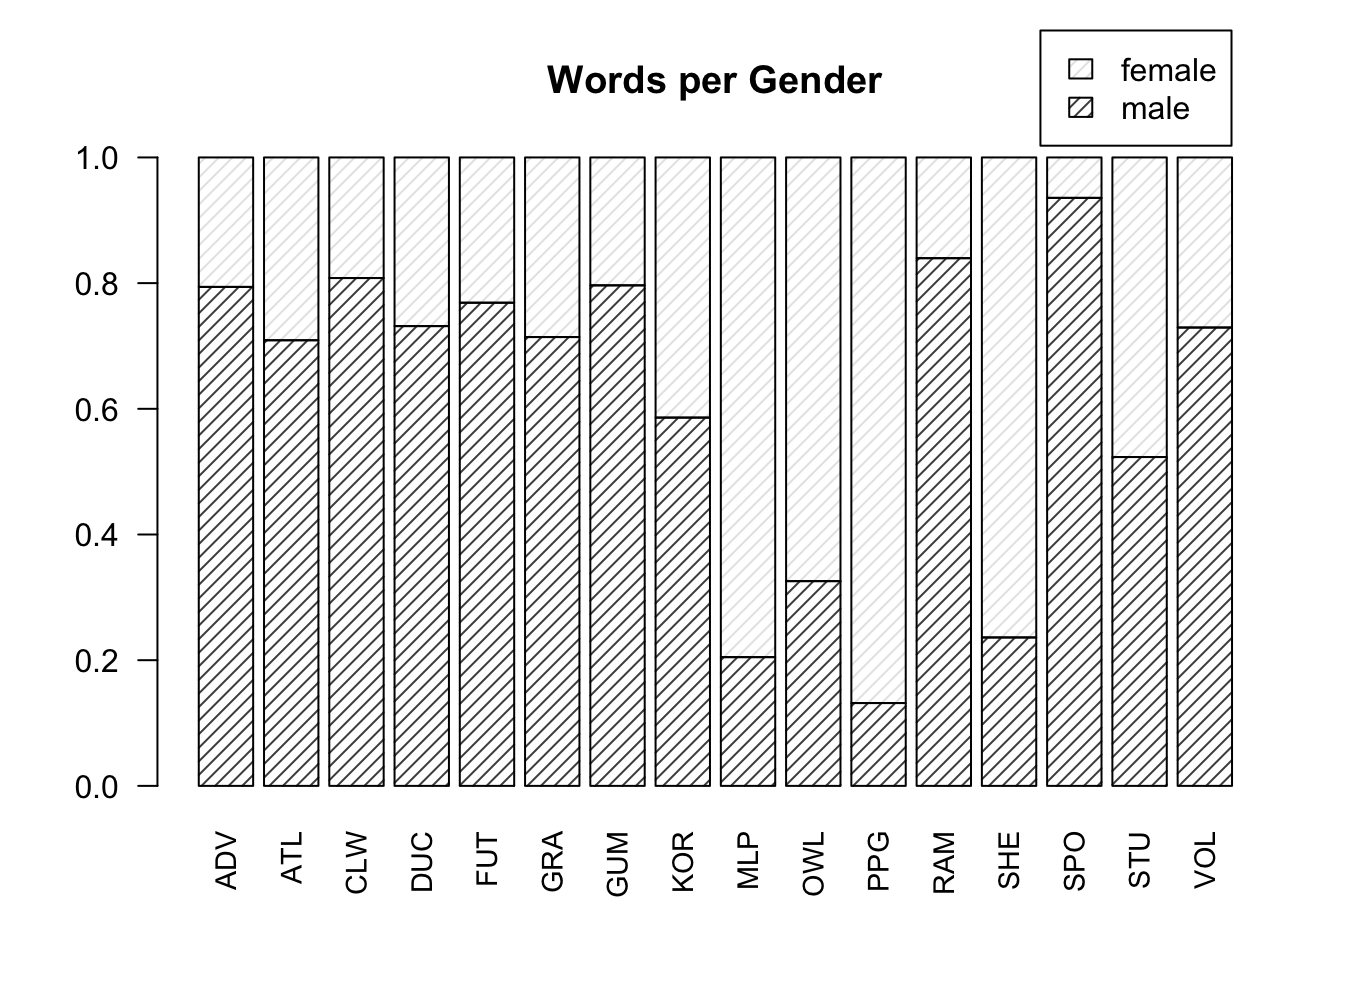
\includegraphics[width=\linewidth]{figures/worpergen.png}
  \caption{A proportional percentage of words spoken by each gender.}
  \label{fig:worpergen}
\end{figure}

According to the results, the ratio fluctuates significantly between different shows, reaching from 0.1 (10\% of words spoken in the television show are spoken by men) to 0.95 (95\% of words spoken in the television show are spoken by men). However, the data does not seem to follow a linear pattern when ranked, and many of the shown bars are clustering around specific values. The most notable would be a value of 0.75, around which many of the ratios congregate. The other, albeit less frequent value, is around 0.2, with only a handful of shows that do not belong to either of those two clusters. This finding is interesting, because while a wide range of ratios could be expected beforehand, the clustering is rather jarring. It is possible that this phenomenon could be caused by the occurrence of main characters in almost every television show -- characters recurring in almost every episode and thus having a large impact on the total number of words. Unless the collection of main characters -- the main cast -- is perfectly balanced in terms of gender, it is possible this has a large influence. To some extent, however, it is possible to measure this influence, specifically with variance (displayed in Figures \ref{fig:variance1} and \ref{fig:variance2}).

\begin{figure}[t!]
  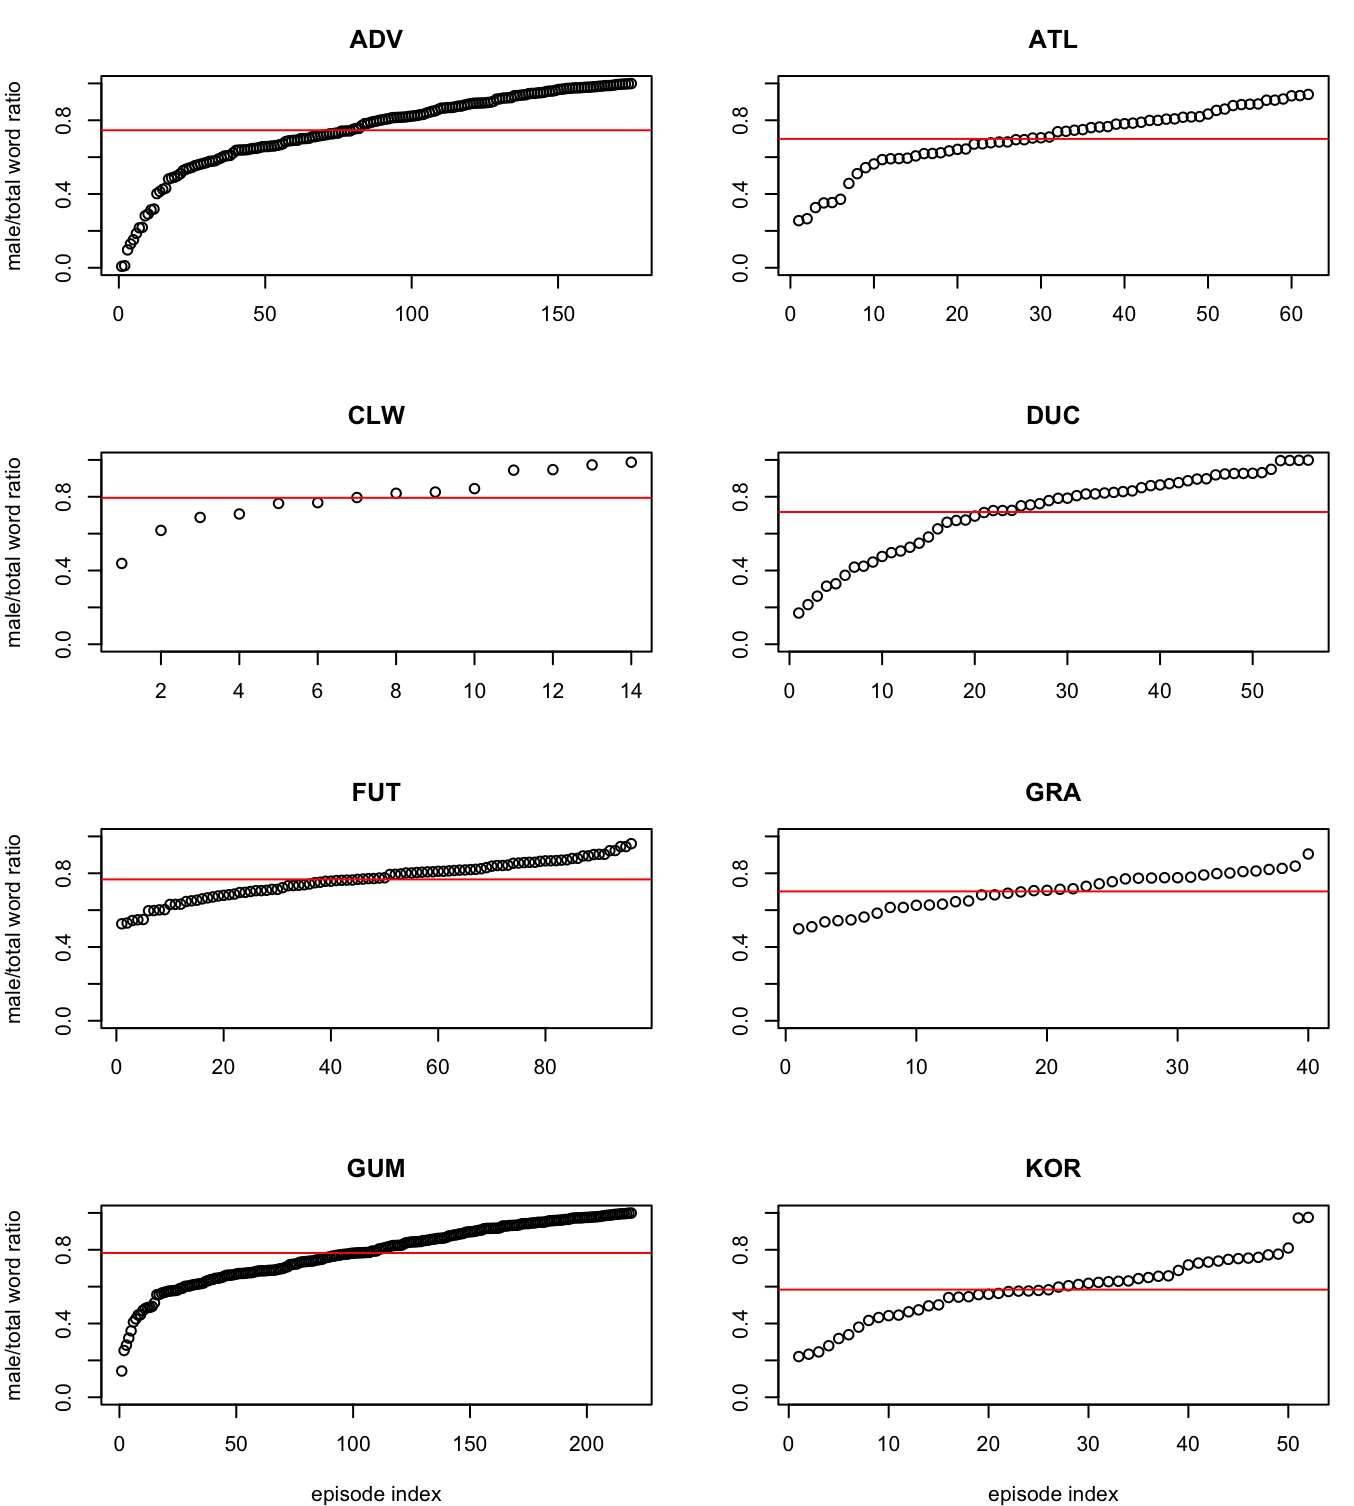
\includegraphics[width=\linewidth]{figures/variance1.png}
  \caption{The ratio of words spoken by male speakers to the total number of words spoken per episode. Individual ranked charts for each cartoon and individual points for each episode with a mean ratio line. Part 1 of 2.}
  \label{fig:variance1}
\end{figure}

\begin{figure}[t!]
  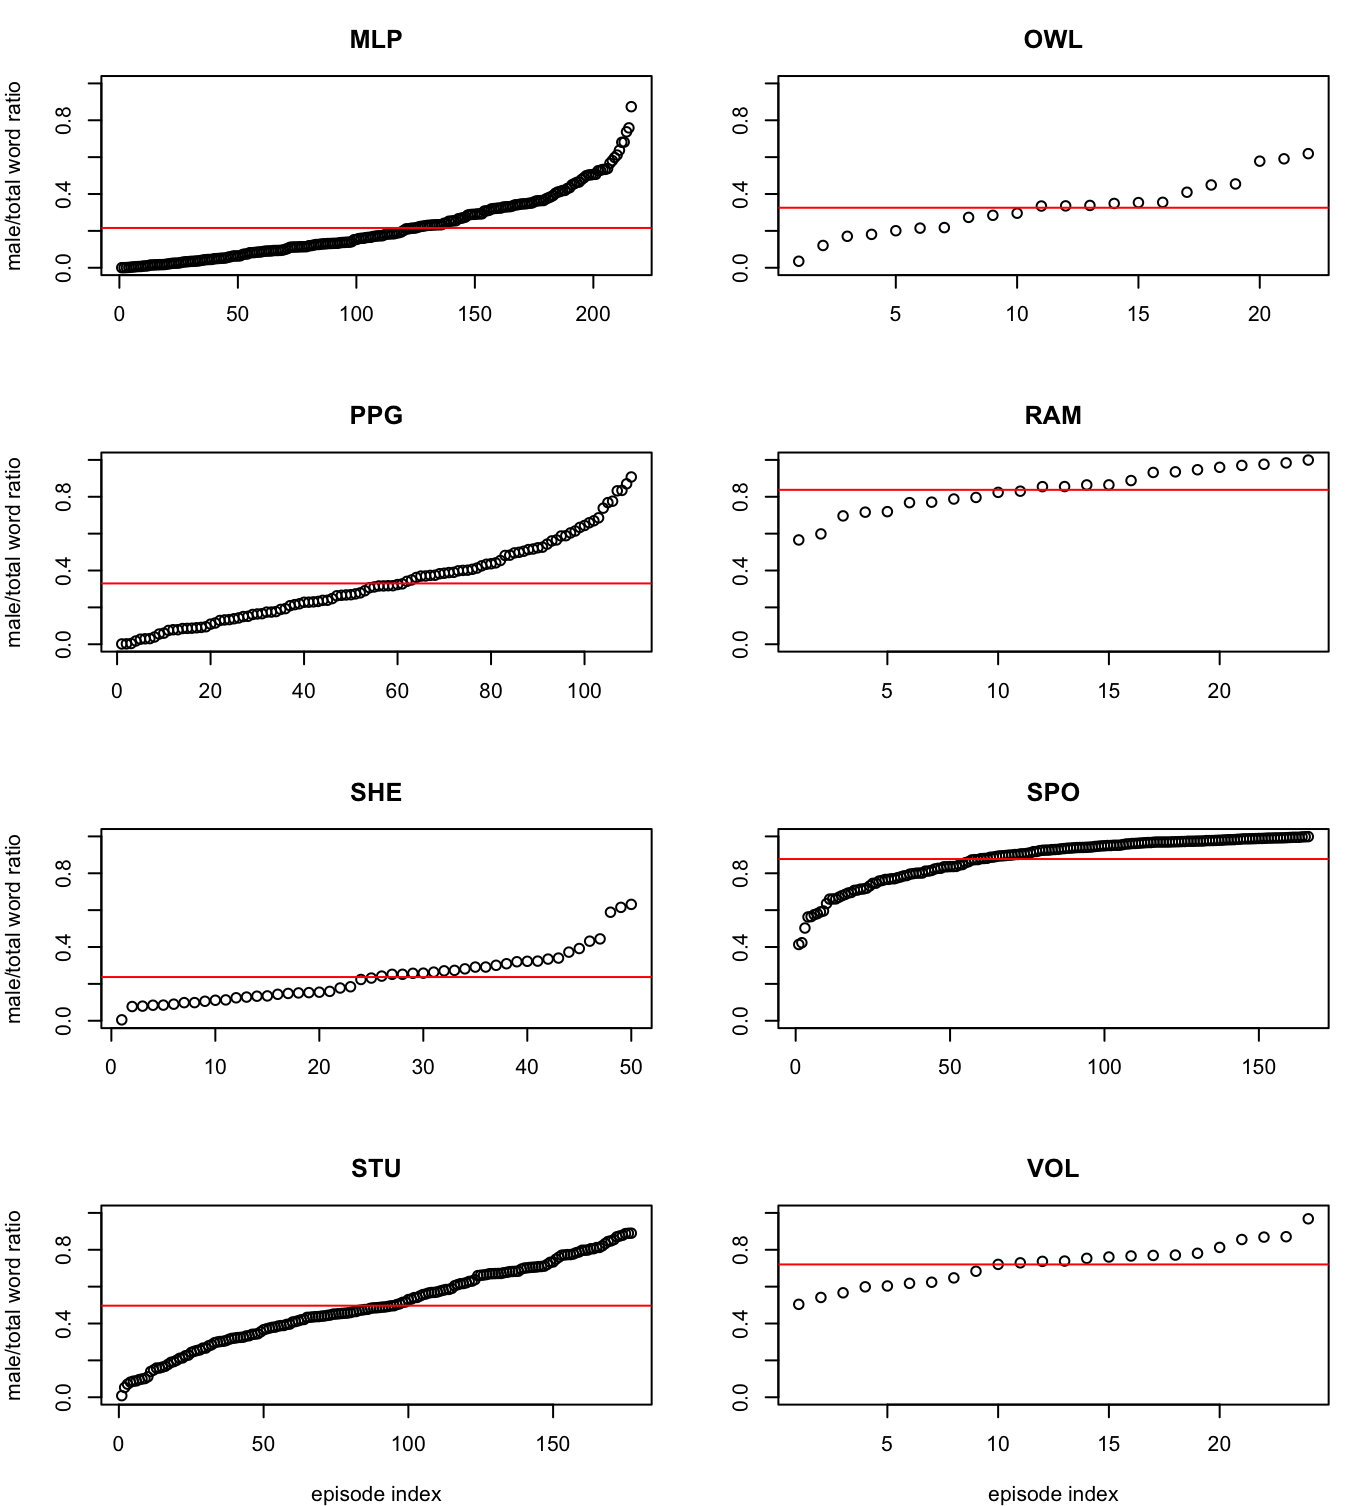
\includegraphics[width=\linewidth]{figures/variance2.png}
  \caption{The ratio of words spoken by male speakers to the total number of words spoken per episode. Individual ranked charts for each cartoon and individual points for each episode with a mean ratio line. Part 2 of 2.}
  \label{fig:variance2}
\end{figure}

For each cartoon, a ranked plot was made with the ratios of male to total words spoken in each individual episode. This statistic is thus an extension of the graph in Figure \ref{fig:worpergen}, merely showing the ratios episode by episode instead of presenting a single value. With a more detailed graph, it is possible to see if individual episode values follow a specific trend -- however, it is important to note that the episodes are ranked by value, not by time of airing, and thus do not speak about the evolution of gender representation over time.

The results are to an extent surprising, as several different patterns can be observed in the different graphs. First off, many of the graphs are relatively linear, but with vastly different skews. It can be deduced that even if two different shows have a similar total ratio, the actual episode-to-episode representation can differ vastly, as some shows feature episodes with mostly the same level of representation each episode (see RAM) and thus closer to the average ratio of the entire show -- represented by a red line in the graphs, while others feature episodes all across the spectrum (see STU). While it is not possible to say that shows with a small skew are highly influenced by their main cast (as the stable nature of their graphs can either be caused by a large influence of the main cast, or a stable level of named-character gender representation outside of it), it is safe to say that shows with a large skew are either to a large extent unaffected by their main cast, or feature many episodes where only a part of the main cast is playing the main role, thus increasing the variance of its gender representation.

However, this is not the only interesting finding in the graphs: several graphs do not seem to follow a linear pattern at all (see ADV, GUM as an example). Instead, their graphs more closely resemble a logarithmic scale, with a relatively stable ratio throughout the majority of the episodes and a trail of either increasing (see SPO) or decreasing (see MLP) female representation -- one that is more significant than an outlier. It is debatable why this occurs, and more data, specifically time of airing data would be required to make any further conclusions. This behavior can be caused by occasional episodes which largely focus on a different set of characters -- although this idea would most likely not result in such pattern, as the episode statistics would more likely cause a jump rather than a gradual increase/decrease. It is also possible this behavior is caused by a change in main cast, or -- if supported by times of airing -- by a gradual move toward a different level of gender representation.

The next statistic in the study is the one of speakers themselves. Moving entirely away from how many words a speaker says over the course of the cartoon (aside from the limitation of a minumum of 100 total words spoken), this statistic (displayed in Figure \ref{fig:spkpergen}) covers the ratio of male speakers versus female speakers for each individual show.

\begin{figure}[t!]
  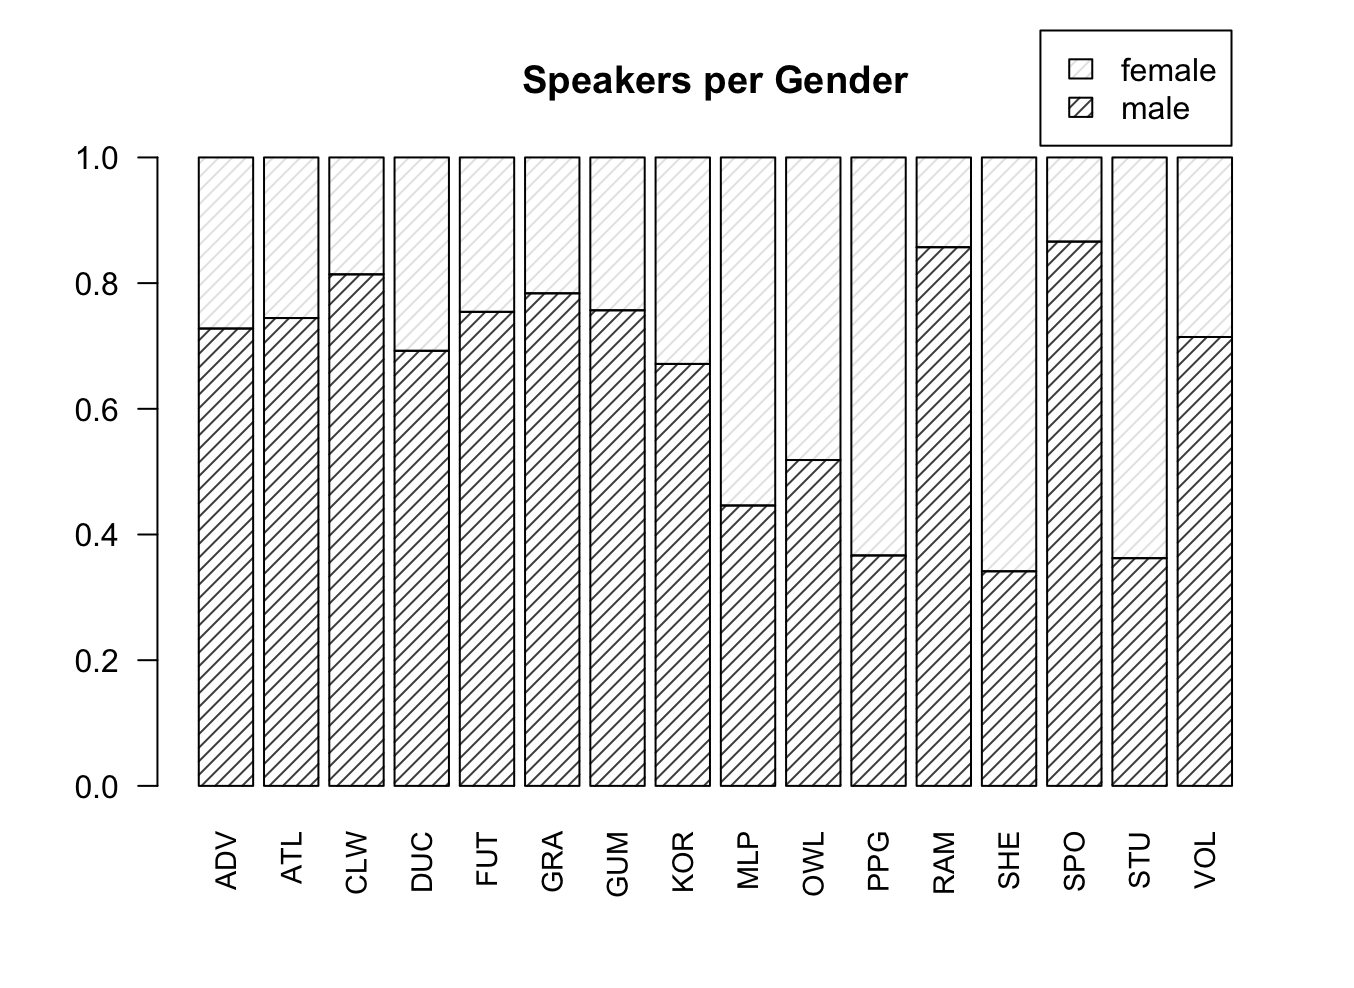
\includegraphics[width=\linewidth]{figures/spkpergen.png}
  \caption{A proportional percentage of speakers of each gender.}
  \label{fig:spkpergen}
\end{figure}

As with the ratio of words spoken by different genders earlier, the data in this graph fluctuate as well, although to a significantly lesser degree, only from about 0.35 to 0.9, showing the ratio is less extreme when only taking into account the speaker numbers themselves. Such a statistic shows some other interesting behaviors, such as the fact that while the ceiling for male representation has not moved much from Figure \ref{fig:worpergen} to this one (only from 0.95 to 0.9), the floor has moved to a much bigger degree (from 0.1 to 0.35). From this, it can be deduced that even when shows consist mainly or almost entirely of lines spoken by one gender, there is still a floor for the minumum number of speakers of each gender, and this floor is higher for male characters. Additionally, the clustering pattern observed in Figure \ref{fig:worpergen} is even more apparent here: all of the displayed shows can be split into two clusters, a larger one centered at around 0.75, and a smaller one clustering at around 0.4. 

\begin{figure}[t!]
  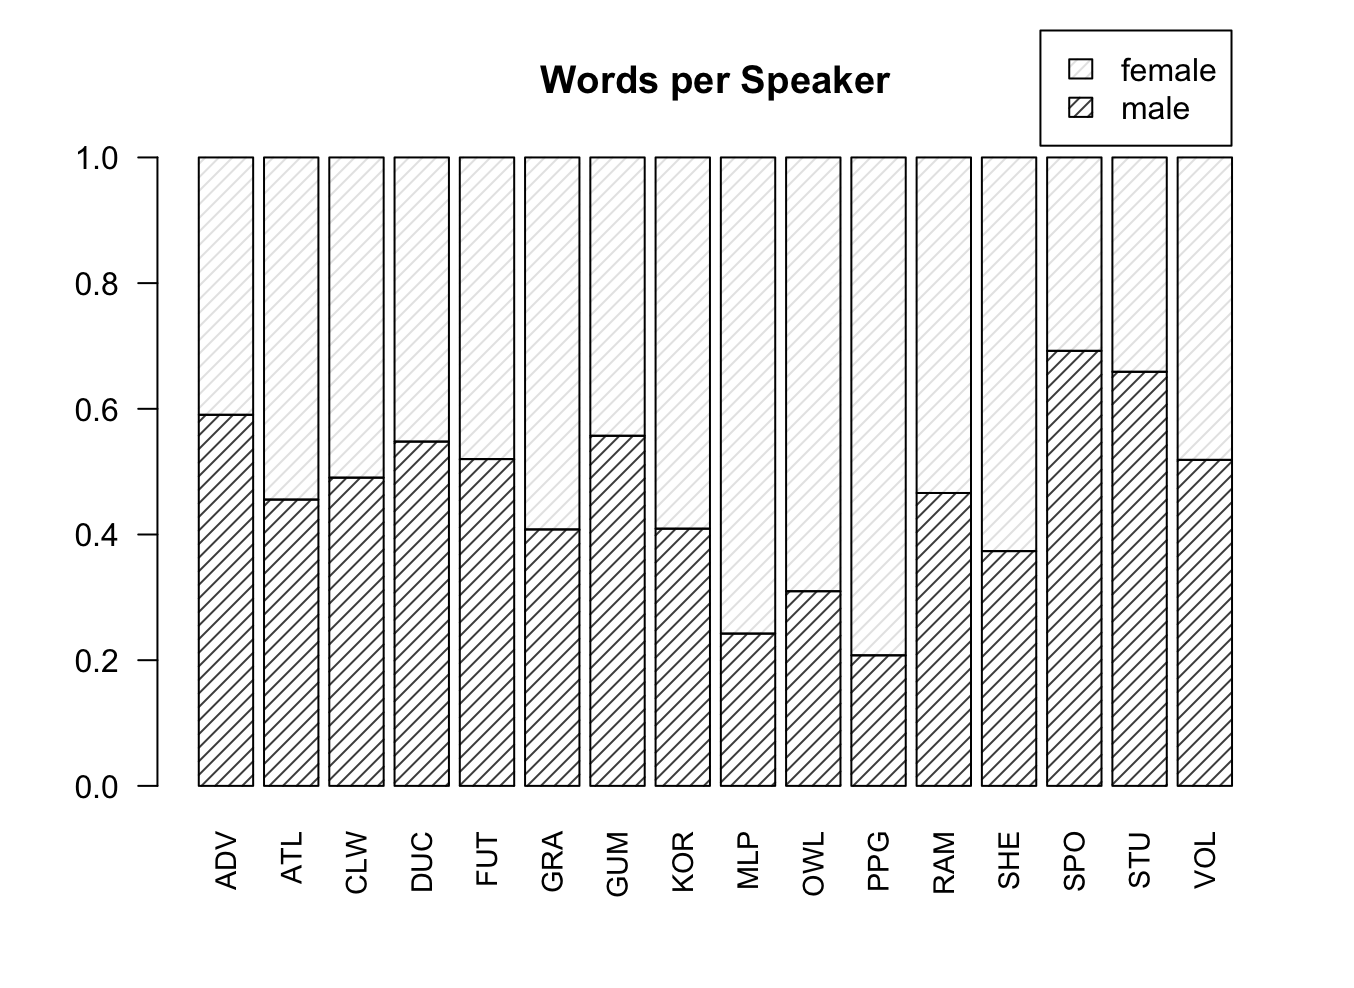
\includegraphics[width=\linewidth]{figures/worperspk.png}
  \caption{A proportional chart of words spoken by each individual speaker.}
  \label{fig:worperspk}
\end{figure}

\begin{figure}[t!]
  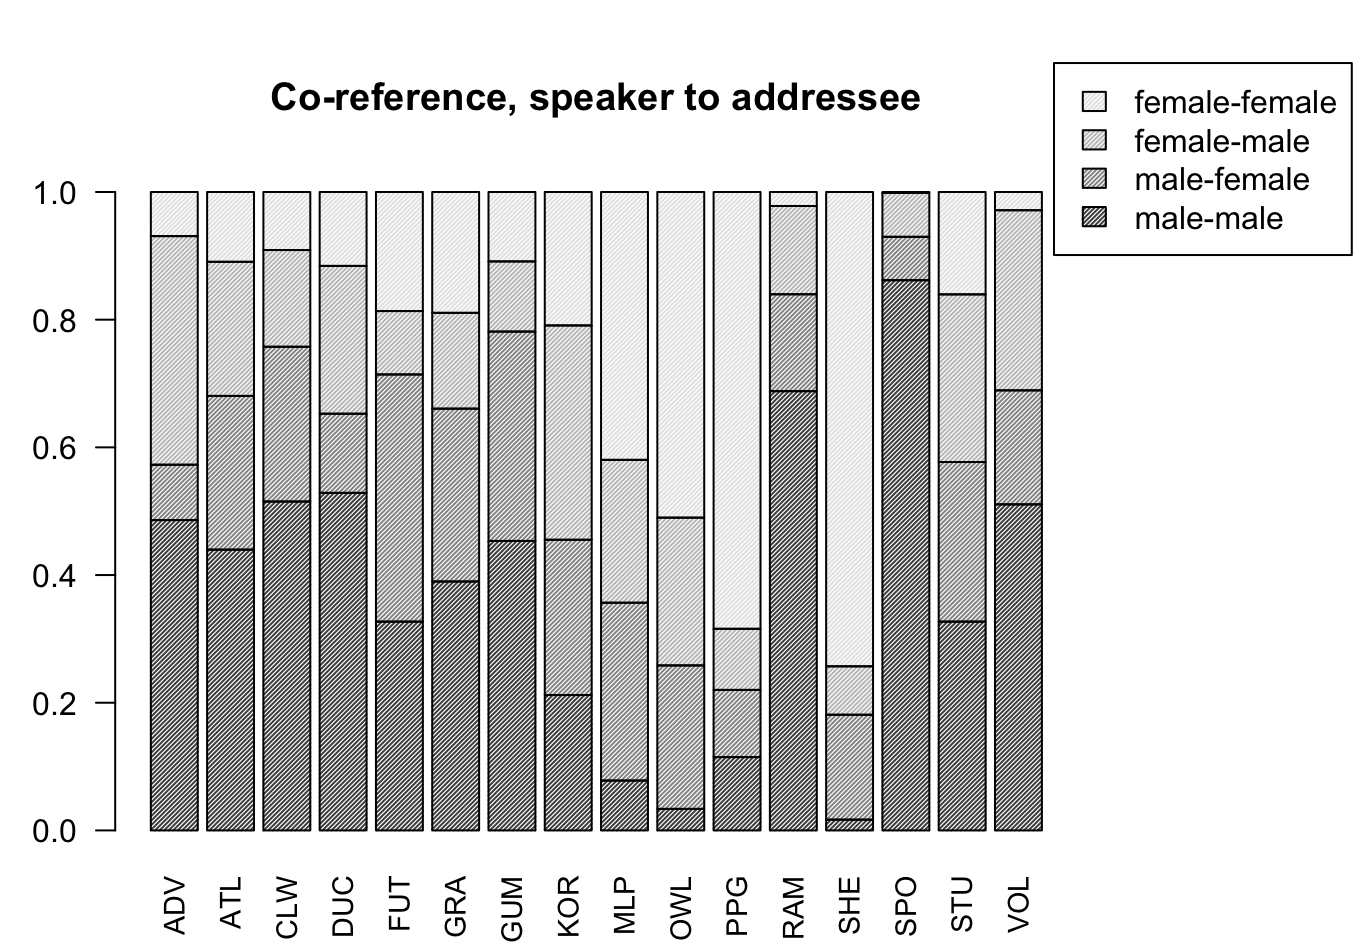
\includegraphics[width=\linewidth]{figures/coreference.png}
  \caption{A co-reference graph, speaker to addressee gender.}
  \label{fig:coreference}
\end{figure}

\section{Conclusion}

\bibliographystyle{chicago}
\bibliography{main}

\end{document}
